\documentclass[pdflatex]{article}
\usepackage[frenchb]{babel}
\usepackage[T1]{fontenc}
\usepackage[latin1]{inputenc}
\usepackage{varioref}
\usepackage{graphicx}
\usepackage[left=2cm,top=1cm,right=2cm,nohead,nofoot]{geometry}

\begin{document}

\title{Visual R reference card (Draft)}

\maketitle

\author Sylvain Loiseau <sylvain.loiseau@unicaen.fr>

Universit\'e de Caen--Basse Normandie

\section{Anatomy of a vector}
% ----------------------------

All elements of a vector have a common mode, one of character, logical, and numeric.

\begin{tabular}{ccc}
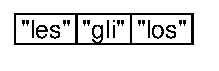
\includegraphics{v_char} & 
\includegraphics{v_log} & 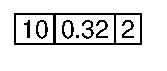
\includegraphics{v_num}\\
\end{tabular}

All elements of a vector have an index. They may have a name.

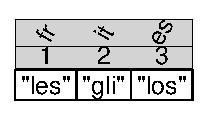
\includegraphics{v_char_names} 

All vectors have two important properties : their mode and their length.

\begin{tabular}{cc}
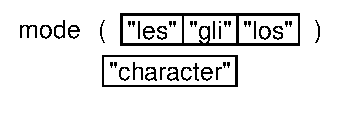
\includegraphics{v_char_type} & 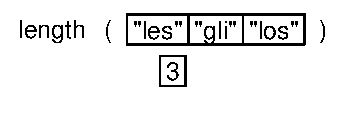
\includegraphics{v_char_length}\\
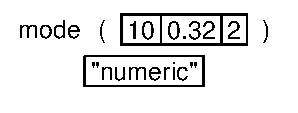
\includegraphics{v_num_type} & 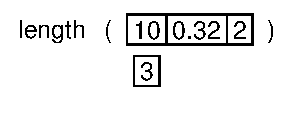
\includegraphics{v_num_length}\\
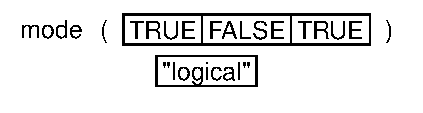
\includegraphics{v_log_type} & 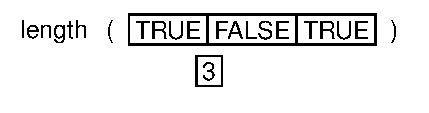
\includegraphics{v_log_length}\\
\end{tabular}

Functions are very precisly defined in terms of mode, number and length of vectors they may take as argument, and mode and length of vector they create.

- length() take one vector of any mode and length and return a vector of numeric vector of length 1.

- mode() take one vector of any mode and length and return a character vector of length 1.


\section{Creating a vector}
% ----------------------------

\begin{tabular}{cc}
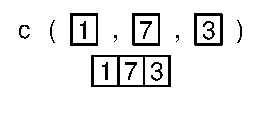
\includegraphics{c_1} & 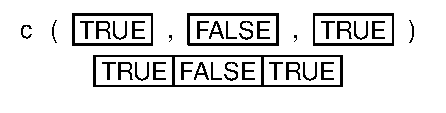
\includegraphics{c_2}\\
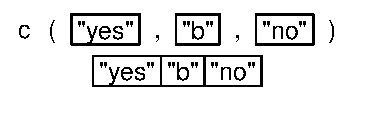
\includegraphics{c_3} & \\
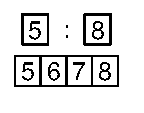
\includegraphics{operator_sequence} & 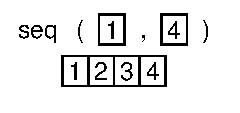
\includegraphics{seq}\\
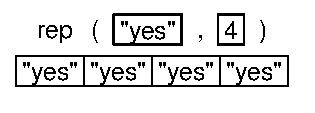
\includegraphics{rep} & 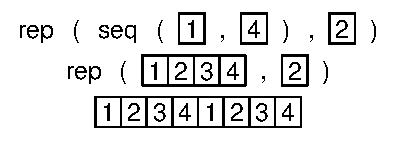
\includegraphics{rep_seq}\\
\end{tabular}

The function c() take any number of vectors of any length and any mode, but all vectors must have the same mode (see below, "Conversion"). It returns a vector of the same mode as the arguments and whose length is the sum of the length of its arguments.

\section{Extraction}
% ----------------------------

A vector can be created by extracting some elements of a vector.

Elements to be extracted can be addressed using their index.

\begin{tabular}{cc}
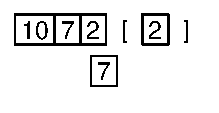
\includegraphics{extract_num} 
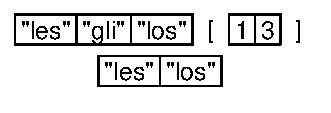
\includegraphics{extract_nums} 
\end{tabular}

Index are 1-based. If an index is greater than the number of element in the vector, you get "NA". If the vector has names, their are preserved.

\begin{tabular}{cc}
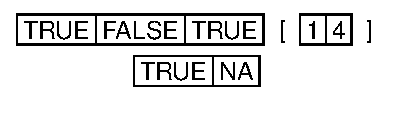
\includegraphics{extract_nums_outsider} & 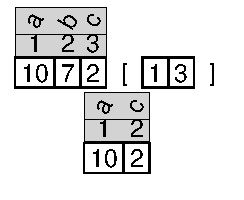
\includegraphics{extract_nums_names}
\end{tabular}

You can also extract with character or logical vector inside the square brackets of the extraction operator. Elements of a character vector are interpreted as the names of the elements to be extracted (elements must have names!).

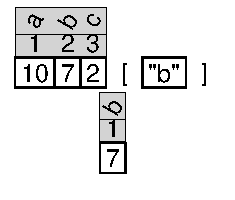
\includegraphics{extract_char_names}

Logical vectors must have the same length as the vector to be extracted. Elements are extracted if there is a "TRUE" value at the same position in the logical vector. (If the logical vector is shorter, it is recycled: right (see below for recycling))

\begin{tabular}{ll}
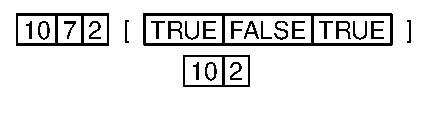
\includegraphics{extract_logical} & 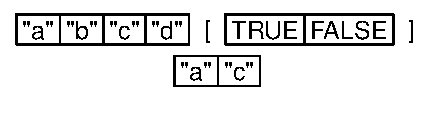
\includegraphics{extract_logical_recycling}\\
\end{tabular}

When extracting, nothing prevent you from reordering elements or extracting  several times the same element:

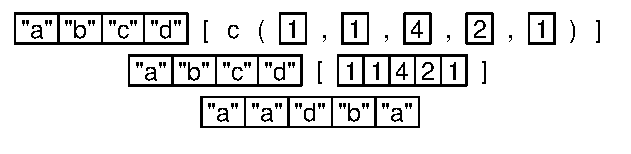
\includegraphics{extract_repeating}

\section{Operator}
% ----------------------------

Some numeric operators.

\begin{tabular}{ccc}
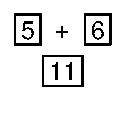
\includegraphics{operator_plus} & 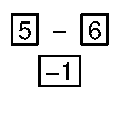
\includegraphics{operator_minus} & 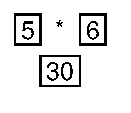
\includegraphics{operator_time}\\
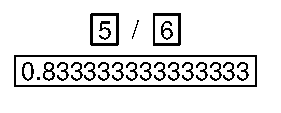
\includegraphics{operator_div} & 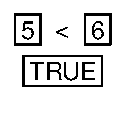
\includegraphics{operator_strict_lt} & 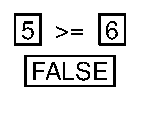
\includegraphics{operator_gt_or_equal}\\
\end{tabular}

Some logical operators.

\begin{tabular}{ccc}
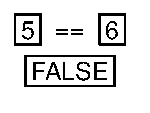
\includegraphics{operator_equality_num} & 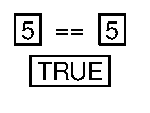
\includegraphics{operator_equality_num_TRUE}\\
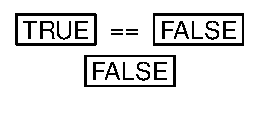
\includegraphics{operator_equality_log} & 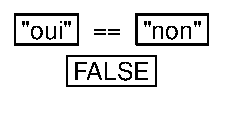
\includegraphics{operator_equality_char}\\
\end{tabular}

\section{Vectorization}
% ----------------------------

Operators -- as well as many functions -- may operate on vector of any length: the operation is performed on pair of elements of equal index.

\begin{tabular}{cc}
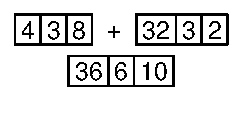
\includegraphics{operator_plus_vectorized} & 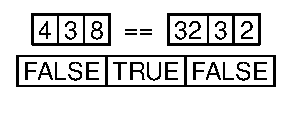
\includegraphics{operator_equal_vectorized}\\
\end{tabular}

\section{Recycling}
% ----------------------------

In a context where vectorization is allowed, you may provide vectors of unequal length. The shorter is duplicated until its length reach the length of the longer. This is called recycling a vector.

\begin{tabular}{cc}
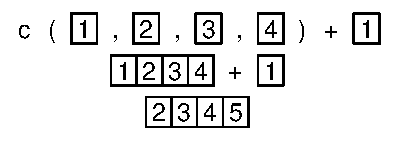
\includegraphics{operator_add} & 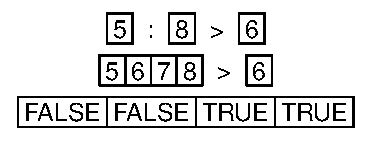
\includegraphics{operator_gt}\\
\end{tabular}

Be careful:

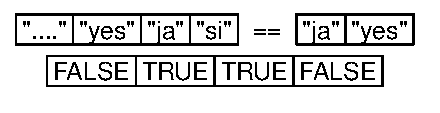
\includegraphics{operator_recycling}

\section{Some numerical functions}
% ----------------------------

Some functions for numeric vectors.

\begin{tabular}{cc}
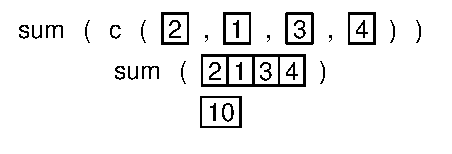
\includegraphics{sum} & 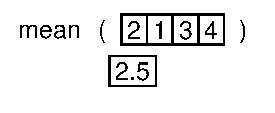
\includegraphics{mean}\\
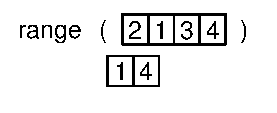
\includegraphics{range} & 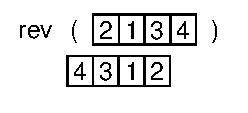
\includegraphics{rev}\\
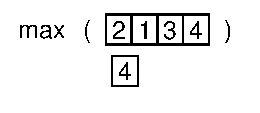
\includegraphics{max} & 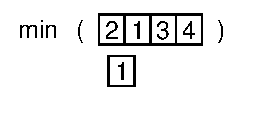
\includegraphics{min}\\
\end{tabular}

%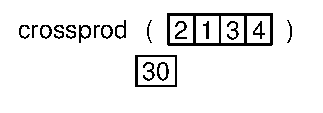
\includegraphics{crossprod}

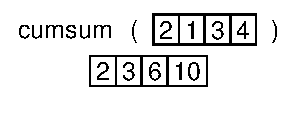
\includegraphics{cumsum}

TODO : table

\section{Some string functions}
% ----------------------------

nchar() count the number of characters in all strings of a character vector.

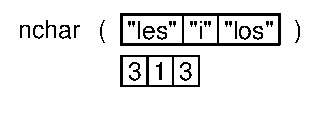
\includegraphics{nchar}

Recycling and vectorization are useful with paste(), which concatenates characters string at same index in several characters vectors:

\begin{tabular}{cc}
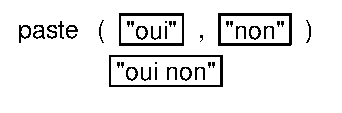
\includegraphics{paste} & \includegraphics{paste2}\\
\includegraphics{paste3} & \includegraphics{paste4}\\
\end{tabular}

You can paste more than two vectors of characters:

\includegraphics{paste5}

\section{Sorting}
% ----------------------------

Numeric and character vectors can be sorted. Names are preserved.

\begin{tabular}{cc}
\includegraphics{sort} & \includegraphics{sort2}\\
\includegraphics{sort_char} & \includegraphics{sort_char_names} \\
\end{tabular}

\section{Type conversion}
% ----------------------------

c() coerce arguments to a common mode -- all elements of a vector always have a common mode.

The character mode always wins. Logical always looses.

\begin{tabular}{cc}
\includegraphics{conversion_1} & \includegraphics{conversion}\\
\end{tabular}

% TODO : more on type conversion. Exemple of functions silently converting their argument. nchar() for instance, on numeric.

\section{Index}
% ----------------------------

Some useful functions give index rather than the actual values.

\includegraphics{which}

\begin{tabular}{cc}
\includegraphics{order} & \includegraphics{order2}\\
\includegraphics{which_min} & \includegraphics{which_max}\\
\end{tabular}

% TODO : This is particularly usefull in very common situation where two or
% more vectors are "aligned", or synchronized, and you don't want to loose the
% initial order

\section{Precedence}
% ----------------------------

Operators have precedence (see ?Syntax).

"seq" takes precedence over "+", "seq" takes precedence over logical operators...

\begin{tabular}{cc}
\includegraphics{precedence} & \includegraphics{operator_gt}\\
\end{tabular}

The order in which the operators are written in the code does not matter!

\includegraphics{operator_gt_inv}

\section{Factor}
% ----------------------------

TODO

There is numerous situations where values of a vector are seen as modalities, allowing for grouping, etc. (split, rowsum, tapply, by, etc.)

\section{Matrix}
% ----------------------------

\subsection{Creation}

Matrix are created with the matrix() function. It takes three main arguments: a
vector (any type and any length) gives the content, two vectors (numeric and
length 1) give the numbers of rows and columns. If only one dimension is given,
the second one is deduced from the length of the vector. If both dimensions are
given and the vector length do not match the number of cells, the vector is
recycled to fill the matrix. The matrix is filled by column; this behavior may
be changed with the option byrow. 

\begin{tabular}{cc}
\includegraphics{matrix} & \includegraphics{matrix_arg}\\
\includegraphics{matrix_byrow} & \includegraphics{matrix_nbcol}\\
\includegraphics{matrix_logical} &
\end{tabular}

\subsection{Extraction with a matrix}

Matrices have two dimensions and you must provide extractors for each of them.
You first extract the rows, then the columns.

\begin{tabular}{cc}
\includegraphics{matrix_extraction} & \includegraphics{matrix_extraction3}\\
\includegraphics{matrix_extraction2} & \includegraphics{matrix_extraction4}\\
\end{tabular}

%\begin{tabular}{cc}
\includegraphics{matrix_extraction5}
%& \includegraphics{matrix_extraction_drop}
%\end{tabular}

How does extraction in a matrix preserve names? No name is preserved if you extract a single element; longuest dimension's names are preserved if you extract a vector of more than one element, both dimensions are preserved if you extract a sub-matrix:

\includegraphics{matrix_extraction8}
\includegraphics{matrix_extraction6}
\includegraphics{matrix_extraction7}

\subsection{Properties}

\begin{tabular}{ccc}
\includegraphics{nrow.pdf} & \includegraphics{ncol.pdf} & \includegraphics{dim.pdf}
\end{tabular}

\begin{tabular}{cc}
\includegraphics{rownames.pdf} & \includegraphics{colnames.pdf}
\end{tabular}

\begin{tabular}{cc}
\includegraphics{length_matrix.pdf} & \includegraphics{mode_matrix.pdf}
\end{tabular}

A matrix is very similar to a vector: it has a mode and a length. It has also
two dimensions and, then, it has two vector of names and it takes two index
vectors inside extraction operator. But you can often see a matrix as a vector.
For instance, if you use only one index vector inside the extraction operator,
it extracts from the underlying, column-filled vector:

\includegraphics{matrix_extraction_as_vector}

\subsection{Summing a matrix}

\includegraphics{matrix_sum} 

\begin{tabular}{ccc}
\includegraphics{rowSums} & \includegraphics{colSums}
\end{tabular}

rowsum() performs a colSums on each group of rows given by the second argument.

\includegraphics{rowsum} 

\subsection{Changing}

\begin{tabular}{cc}
\includegraphics{as_vector} & \includegraphics{matrix_operator}\\
\end{tabular}

\begin{tabular}{cc}
\includegraphics{cbind.pdf} & \includegraphics{rbind.pdf}\\
\end{tabular}

\includegraphics{merge.pdf} 

\includegraphics{t.pdf} 

\section{list}
% ----------------------------

\subsection{Creation, anatomy}

Creating a list by enumerating its components.

A list of length 4: contains 4 vectors, each of length 1 (left) ;
a list of length 1: contains 1 vector of length 2 (right).

\begin{tabular}{cc}
\includegraphics{list_enumerate.pdf} & \includegraphics{list_onetype.pdf}
\end{tabular}

% Same as above
% 
% \includegraphics{list.pdf}

List can contain objects of different mode (left) ;
it can contain objects of different dimensions (right).

\begin{tabular}{cc}
\includegraphics{list_twotypes.pdf} & \includegraphics{list_matrix.pdf}
\end{tabular}

A list can be recursive: a component may be a list.

\includegraphics{list_complex.pdf}

% \includegraphics{list_rec.pdf}

\subsection{Basic functions}

TODO...

\includegraphics{list_names}

\includegraphics{list_length}

\includegraphics{list_mode}

\subsection{Extraction}

Extracting in a list. The next two figures show the difference beween [ and [[ operator on list: the first create a sublist (it extracts elements, exactly as it extracts elements from a vector), while the second is completely different: it give the content of one (and only one) element of a list.

\begin{tabular}{cc}
\includegraphics{list_extract_simple.pdf} & \includegraphics{list_extract_double.pdf}
\end{tabular}

You can use vector of any length within the single-square bracket, while you can address only one element within the double-square-bracket operator, and then use only vector of length 1.

Since a list is a recursive data structure (may contain list), you can use several successive bracket operators in order to go down to the element you're interested in.

With the single-square-bracket operator you cannot walk down though the data structure.

\includegraphics{list_successive_extraction}

\subsection{List and vector}

\begin{tabular}{cc}
\includegraphics{unlist} & \includegraphics{aslist}
\end{tabular}


\subsection{List for expressing complex data structure}

Grouping elements of a vector using a the level of a factors:

\includegraphics{split}

See also for instance strsplit() below.

\section{Regexp}

\subsection{Split strings: strplit()}

\includegraphics{strsplit.pdf}

\includegraphics{strsplit_2.pdf}

\subsection{Extract sub strings: substr()}

\includegraphics{substr.pdf}

\includegraphics{substr_2.pdf}

\includegraphics{substr_3.pdf}

\subsection{Searching elements of a character vector with regexp: grep()}

\includegraphics{grep}

\includegraphics{grepl}

\subsection{Substitution: sub()}

\includegraphics{sub}

\includegraphics{gsub}

\subsection{Searching substring in elements of character vector: regexpr()}

TODO

\section{Data Frame}

TODO

% \section{apply}
% 
% mapply eapply tapply sapply lapply rapply
% tapply avec range
% by sweep
% lier à factor
% 
% \section{set}
% union(...) unique
% any, all
% 
% 
% \section{Other}
% 
% pmatch
% 
% 
% %MATRIX
% %col
% %margin.table
% %slice.index
% split
% %class.ind ? dans package nnet
% %max.col, max.row
% 
% TESTER EGALIT1
% match => %in%
% identical
% switch ifelse
% 
% cut
% 
% labels

% switch

\end{document}
